%http://www.cs.put.poznan.pl/ksiek/latexmath.html
%https://en.wikibooks.org/wiki/LaTeX/Advanced_Mathematics


\documentclass[a4paper]{article} 
\usepackage[T1]{fontenc} 
\usepackage[utf8]{inputenc} 
\usepackage[fleqn]{amsmath}
\usepackage{amssymb}
\usepackage{cancel}
\usepackage{graphicx}
\usepackage{enumitem}
\usepackage{systeme}
\usepackage{environ}
\usepackage{color}
\definecolor{javared}{rgb}{0.6,0,0} % for strings
\definecolor{javagreen}{rgb}{0.25,0.5,0.35} % comments
\definecolor{javapurple}{rgb}{0.5,0,0.35} % keywords
\definecolor{javadocblue}{rgb}{0.25,0.35,0.75} % javadoc

\usepackage{listings}
\lstset{
	basicstyle=\ttfamily,
	keywordstyle=\color{javapurple}\bfseries,
	stringstyle=\color{javared},
	commentstyle=\color{javagreen},
	morecomment=[s][\color{javadocblue}]{/**}{*/},
	tabsize=4,
	showspaces=false,
	showstringspaces=false}

\usepackage[top=1in, bottom=1.25in, left=1.0in, right=1.25in]{geometry}

\setlength{\parindent}{0em}
\setlength{\parskip}{1em}

\newenvironment{task}[1]
{
	\begin{description}[align=right]
		\item [#1]
}{		%input
	\end{description}
}

\newcommand{\abs}[1]{\left|#1\right|}

\newcommand{\taskref}[1]{\textbf{#1}}

\DeclareMathOperator{\lra}{\ \Leftrightarrow\ }
\DeclareMathOperator{\llra}{\ \longleftrightarrow\ }
\DeclareMathOperator{\ra}{\ \Rightarrow\ }
\DeclareMathOperator{\OPT}{OPT}

\let\*\relax
\DeclareMathOperator{\*}{\cdot}

\title{Algoritmer, datastrukturer och komplexitet\\ EDAF05} 
\author{Emil Wihlander\\ dat15ewi@student.lu.se} 

\begin{document} 
\maketitle

\section*{Exam 140526}
\subsection*{Analysis of algorithms}

\begin{task}{1. (a)}
	\framebox{A} Because $N$ needs to be twice as big every time you want to print one more star the algorithm has logarithmic growth.
\end{task}

\begin{task}{(b)}
	\framebox{D} The function f will call g $N$ times which means g will print $0, 1, \ldots, N$ stars. The total number of stars will therefore be the sum of that serie of numbers. The formula for arethmetic sums is $N\*(0+N)/2=(1/2)\*N^2$ which give it an order of $O(N^2)$.
\end{task}

\subsection*{Divide-and-conquer}

\begin{task}{2. (a)}
	\framebox{A} Subtree, you can easily break it down into subproblems by recursively solving it for the children. The conquer part is a bit more tricky. You need to save both the largest perfect subtree (lps) and the largest perfect subtree with the top node as base (tps). With that information you can calculate the lps and tps one level up, see \taskref{(b)}. 
\end{task}

\begin{task}{(b)}
	\qquad The following function solves it by a recursive divide-and-conquer algorithm. \texttt{Subtree} is a class that contains the largest perfect subtree (\texttt{.lps()}) and the largest perfect subtree with the top node as base (\texttt{.tps()}). \texttt{TreeNode} contains the children (\texttt{.left()} and \texttt{.right()}).
\begin{lstlisting}[language=Java]
private Subtree f(TreeNode node) {
	// base case
	if (node == null) 
		return new Subtree(0, 0)
	// DIVIDE
	Subtree left = f(node.left());
	Subtree right = f(node.right());
	// CONQUER
	// Builds the new top perfect subtree (tps)
	int tps = 1 + Math.min(left.tps(), right.tps());
	// Finds the new largest perfect subtree (lps)
	int lps = Math.max(left.lps(), right.lps(), tps);
	
	return new Subtree(x, y);
}
\end{lstlisting}
\end{task}

\begin{task}{(c)}
	\framebox{B} Since there are no cycles it will traverse through each node exactly once. The conquer step is $O(1)$ which means the algorithm will run in $O(n)$ where $n$ is the number of nodes.
\end{task}

\subsection*{Graph connectivity}

\begin{task}{3. (a)}
	\framebox{B} Clearance, see \taskref{(b)} for explanation.
\end{task}

\begin{task}{(b)}
	\qquad Start with an empty graph, add each $w\in E$ in ascending order until there is a connection between $s$ and $t$. If you use Breadth-first search for finding a connection the worst case performance for each iteration is $0, 2, 4, \ldots , 2\*n$ the aretmethic sum is $2\sum_{k=0}^{n}k=2\*n^2/2=n^2$ the order is therefore $O(n^2)$.
\end{task}

\subsection*{Dynamic programming}

\begin{task}{4. (a)}
	\framebox{C} Long. Since we know all edges are directed from left to right we analyze all vertices from left to right. The value for each vertex will be the value of the max of all past vertices that is connected (if none is, assign value 0) to the current vertex plus one, and that is the dynamic programming part. 
\end{task}

\begin{task}{(b)}
	\framebox{C} The problem is one-dimensional and therefore only one of the $OPT(i)$ options can be correct (\framebox{C} or \framebox{G}). The past vertices you should compare are depented on which edges exist rather than vertices with the same iterative distance. \framebox{C} is therefore the only possible option. 
\end{task}

\begin{task}{(c)}
	\framebox{B} The algorithm will iterate through all vertices, $n$, and edges, $m$, exactly once ($n+m$). The maximum number of incoming edges is for $v_1=0, v_2=1, \ldots, v_n=n-1$ which gives the aretmethic sum of $m\leq (n-1)^2/2$ which is larger than $n$ for large values. The order of the algorithm is therefore $O(m)$.
\end{task}

\begin{task}{(d)}
	\framebox{A} You will save one value per vertex (maximum path length to current vertex) and the space order will therefore be $O(n)$.
\end{task}

\subsection*{Network flow}

\begin{task}{5. (a)}
	\framebox{D} V, you can look at this as a maximum flow problem, see \taskref{(b)} for futher explanation.
\end{task}

\begin{task}{(b)}
	\qquad Let $L$ be the first column of vertices and $R$ the second column vertices. Then add the edges from the original problem and set their weight to 1, add edges from $s$ to all vertices in the first column with the weight 2 and finally add edges from all vertices in the second column to $t$ with the weight 1.
	
	If the maximum flow equals $2n$ there is a solution, otherwise not. The example from the problem definition is visualized below.
	
	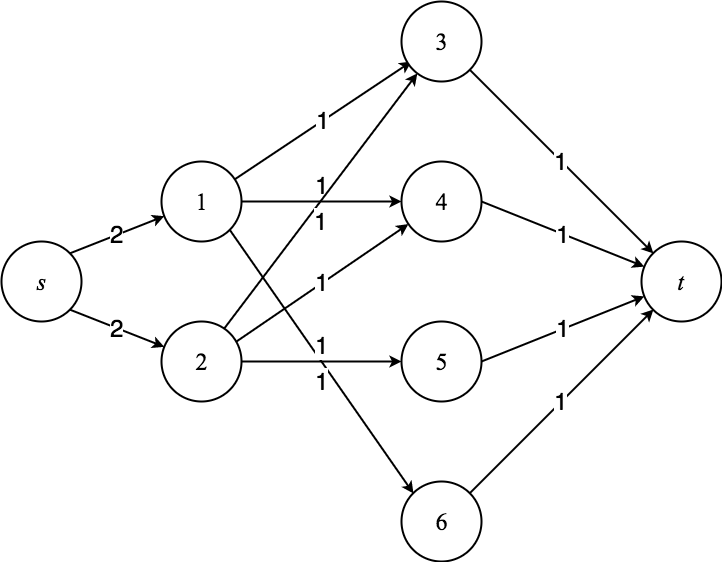
\includegraphics[scale=0.3]{140526-5b.png}
\end{task}

\begin{task}{(c)}
	\framebox{D} As seen in \taskref{(b)}, the number of nodes is $n+m+2\ra O(n+m)$
\end{task}

\subsection*{Computational complexity}

\begin{task}{6. (a)}
	\framebox{E} Crossing, the specific case of when $k=0$ is the Hamiltonian path problem which means Crossing is at least as hard. Hamiltonian path problem is NP-complete which therefore means Crossing is at least NP-complete as well.
\end{task}

\begin{task}{(b)}
	\framebox{H} See \taskref{(a)}.
\end{task}

\begin{task}{(c)}
	\framebox{B} ``The easiest way to see that is to take the following NP-hard problem, Hamiltonian path, and prove that Crossing is at least as hard as Hamiltonian path (Hamiltonian path $\leq_p$ Crossing)''
\end{task}

\begin{task}{(d)}
	\qquad Given an instance to problem Hamiltonian path, $H$, consting of $G(V,E)$, construct an instance of Crossing, $C$, consting of $G'(V',E'), k$. Let $G=G'$ and $k=0$. This reduction runs in constant time.
	
	If $T$ is a solution to $H$ it's also a solution to $C$. Hence Hamiltonian path $\leq_p$ Crossing.
\end{task}

\pagebreak
\section*{Exam 130529}
\subsection*{Analysis of algorithms}

\begin{task}{1. (a)}
	\framebox{C} The code in the \texttt{if} clause has the running time $O(n^2)$ and the code in the \texttt{else} clause has $O(n)$. Since the code block has the running time $O(n^2)$ for large integers that is the answer.
\end{task}

\begin{task}{2. (a)}
	\framebox{A} The opposite argument can be made here. Since the code block has the running time $O(n)$ for large integers that is the answer.
\end{task}

\subsection*{Greedy}

\begin{task}{3. (a)}
	\framebox{A} Buildstacks, you can solve this by using the greedy condition ``always take the coin with the highest value'' and then filling the stacks, starting with $S_1$, then $S_2$ and so on, until you run out of coins.
\end{task}

\begin{task}{(b)}
	\framebox{A} See \taskref{(a)}.
\end{task}

\begin{task}{(c)}
	\framebox{B} See \taskref{(a)}.
\end{task}

\begin{task}{(d)}
	\begin{tabular}{r l}
		$S_1$ & $150,125,125$ \\ \hline
		$S_2$ & $100,100,75$ \\ \hline
		$S_3$ & $50,50,38$ \\ \hline
		$S_4$ & $25$ \\ 
	\end{tabular}
\end{task}

\begin{task}{(e)}
	\framebox{A} The only thing the algorithm has to do is sort the coins in descending order and then you have all your stacks lined up one after the other. This means the algorithm depends on the number of coins, $n$, and not the stack size, $m$.
\end{task}

\subsection*{Graph connectivity}

\begin{task}{4. (a)}
	\framebox{D} Rotten, let each stack be a node and if two stacks have a common type of coin there is an edge between them. If all nodes are connected the disease will spread to all stack regardless of what coin you choose, otherwise not.
\end{task}

\begin{task}{(b)}
	\qquad The example instance is non-solvable since all nodes aren't connected. 
	
	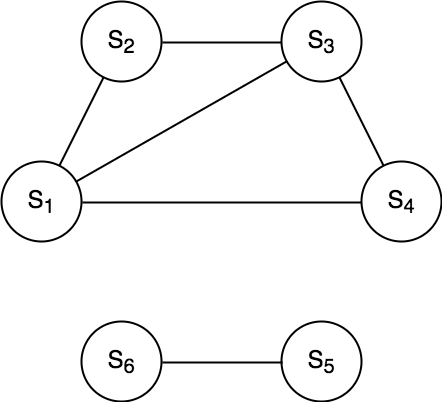
\includegraphics[scale=0.3]{130529-4b.png}
\end{task}

\begin{task}{(c)}
	\framebox{B} See \taskref{(a)}.
\end{task}

\begin{task}{(d)}
	\framebox{C} The first one isn't correct since the shortest path isn't relevant to this problem. The second one isn't correct either since the edges aren't weighted, and an unweighted graph can't have negative cycles which means the last one is false as well. The third one is correct because both Prim's algorithm and BFS (Breadth-first search) finds a minimal spanning tree (if the number of nodes in the tree equals $m$ there is a solution). Prim's running time is $O(m+n \log n)$ and BFS's is $O(m+n)$ where $m$ is the number of nodes and $n$ is the number of edges, BFS is therefore faster.
\end{task}

\begin{task}{(e)}
	\framebox{A} If BFS is used the running time is $O(n+m)$. \footnote{The answer is correct if $m$ represent the number of nodes and $n$ the number of edges. This is not the case since $n$ represents the number of coins types which isn't necessarily the same as number of edges. This is a misstake according to Thore and $n$ should seen as the number of edges.}
\end{task}

\subsection*{Dynamic programming}

\begin{task}{5. (a)}
	\framebox{B} Neighbours, you can iterate, $i$, from left to right where the maximum amount you can take up to the current coin is dependent only on the coins to the left and what the maximum amount at each of those coins is.
\end{task}

\begin{task}{(b)}
	\framebox{G} The optimal solution is the maximum of either the optimal solution for the coin to the left or the current coin value plus the optimal solution for the coin two place to the left.
	
	The example has the following solution (the image is missing a 5 between the 25 and 1, see input/output box at end):
	\begin{align*}
		\OPT(1)=&\max\{\OPT(0), \OPT(-1)+100\}=\max\{0,100\}=100 \\
		\OPT(2)=&\max\{\OPT(1), \OPT(0)+50\}=\max\{100,50\}=100 \\
		\OPT(3)=&\max\{\OPT(2), \OPT(1)+100\}=\max\{100,200\}=200 \\
		\OPT(4)=&\max\{\OPT(3), \OPT(2)+50\}=\max\{200,150\}=200 \\
		\OPT(5)=&\max\{\OPT(4), \OPT(3)+150\}=\max\{200,350\}=350 \\
		\OPT(6)=&\max\{\OPT(5), \OPT(4)+125\}=\max\{350,325\}=350 \\
		\OPT(7)=&\max\{\OPT(6), \OPT(5)+25\}=\max\{350,375\}=375 \\
		\OPT(8)=&\max\{\OPT(7), \OPT(6)+5\}=\max\{375,355\}=375 \\
		\OPT(9)=&\max\{\OPT(8), \OPT(7)+1\}=\max\{375,376\}=376 \\
		\OPT(10)=&\max\{\OPT(9), \OPT(8)+75\}=\max\{376,450\}=450
	\end{align*} 
	This is the maximum sum while the output should be which coins to pick, you can easily sovle that by saving the path the algorithm takes. 
\end{task}

\begin{task}{(c)}
	\framebox{A} As seen in \taskref{(b)}, you need to traverse each coin exactly once.
\end{task}

\subsection*{Network flow}

\begin{task}{6. (a)}
	\framebox{E} Strike, the children shall ``flow'' through the hosts who have a capacity, attributes typical to Network Flow.
\end{task}

\begin{task}{(b)}
	\qquad The first row is all the chilren and the second is all the hosts. The edges between children and hosts are defined by the relationships. the weight between each host and the sink should be the hosts capacity and all other weights should be 1.
	
	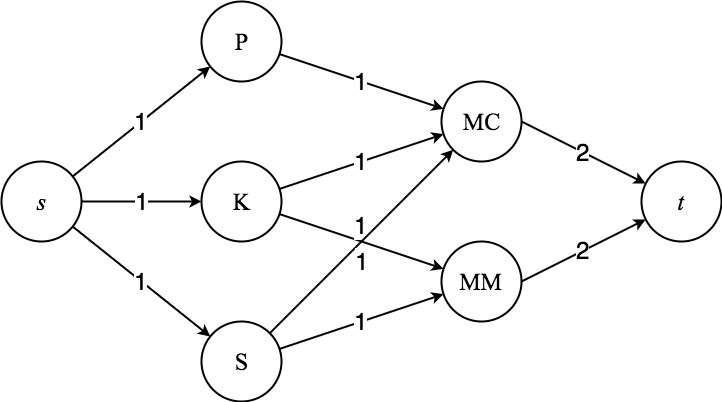
\includegraphics[scale=0.3]{130529-6b.png}
\end{task}

\begin{task}{(c)}
	\framebox{D} the number of nodes is $n+m+2$, see \taskref{(b)}.
\end{task}

\subsection*{Computational compexity}

\begin{task}{7. (a)}
	\framebox{C} Takestacks, let each stack be a node and if two stacks have a common type of coin there is an edge between them. Takestacks then becomes a maximum independent set problem, which is NP-hard.
\end{task}

\begin{task}{(b)}
	\framebox{C} It is a maximum independent set problem.
\end{task}

\begin{task}{(c)}
	\framebox{B} ``The easiest way to see that is to take the following NP-hard problem, Independent set, and prove that Takestacks is at least as hard as Independent set (Independent set $\leq_p$ Takestacks)''
\end{task}

\begin{task}{(d)}
	\qquad Given an instance to problem Independent Set, $I$, consisting of $G(V,E)$. We construct an instance of Takestacks with $m=\abs{V}$ stacks as follows: 
	
	For each vertex $v_i\in V,i=1,2,\ldots,\abs{V}$, we construct a stack $S_i$. For each edge $\{v_i,v_j\}\in E$, we insert a coin of the same unique arbitrary value in stacks $S_i$ and $S_j$. We now have coin values $c_1,c_2,\ldots,c_n,n=\abs{E}$. This reduction runs in linear time.
	
	If $T(S_1,S_2,\ldots,S_m,c_1,c_2,\ldots,c_n)$ is a solution to Takestacks, $T$ is also a solution to the Independent set problem $I$.
	Hence Independent Set $\leq_p$ Takestacks
\end{task}

\pagebreak
\section*{Exam 120523}
\subsection*{Analysis of algorithms}

\begin{task}{1. (a)}
	\framebox{A} For each factor you analyze which term is dominant for large $n$'s ($n^3$ is more dominant than $n^2$). 
\end{task}

\begin{task}{(b)}
	\framebox{B} $O(n^3\log n)\neq O(n^3/\log n)$
\end{task}

\begin{task}{(c)}
	\framebox{B} $O(n^3\log n)\neq O(n^3)$
\end{task}

\begin{task}{2. (a)}
	\framebox{C} The inner most for-loop runs in constant time (can be written \texttt{print "12345678910"}) which means the code blocks order is $O(n^2)$.
\end{task}

\begin{task}{3. (a)}
	\framebox{A} Every time \textbf{remove($S$)} gets called $\abs{S}=1$ since each element that gets inserted is removed directly afterwards. This means both \textbf{remove($S$)} and \textbf{insert($i,S$)} will run in $O(1)$ here. The running time therefore is $O(n)$.
\end{task}

\begin{task}{(b)}
	\framebox{B} The size of $S$ linearly goes from 1 to $n/2$. The upper bound can clearly be set to $O(n\log n)$ (if  $\abs{S}=n$ is true for every iteration and \textbf{remove($S$)} gets called every iteration). To set a lower bound we look at the last half of the sum (from $i=n/2$ to $n$) and lower the bound for each summand to $\log (n/2)=\log (n)-c$ which means the sum is at least $\frac{1}{2}\*\frac{1}{2}\*n\*(\log(n)-c)$. That’s $\Omega(n\log n)$.
\end{task}

\begin{task}{4. (a)}
	\framebox{A} This is the correct option since this should represent the running time. Even though the algorithm takes the maximum of the two you need to calculate both which takes $T(n-1)+T(n-2)$ time. Checking $n > 1$, calculate $\max(x,y)$ and returning 1 takes constant time ($O(1)$).
\end{task}

\begin{task}{5. (a)}
	\framebox{A} Since $L$ and $R$ are the only sets in $B_{l,r}$ the total number of vertices are $l+r$.
\end{task}

\begin{task}{(b)}
	\framebox{C} Each node in $L$ will have $r$ number of edges which means the total is $lr$.
\end{task}

\begin{task}{(c)}
	\framebox{B} No two nodes in $L$ will have an edge nor two nodes in $R$. All nodes in $L$ have edges with all nodes in $R$. This means the answer is either $l$ or $r$.
\end{task}

\begin{task}{(d)}
	\framebox{C} If $l+r\leq 3$ either $r=1$ or $l=1$ since $L$ and $R$ are nonempty sets. The solo node can then be seen as an root to a tree the other nodes as children.
\end{task}

\subsection*{Greedy}

\begin{task}{6. (a)}
	\qquad Consider the following input:
\begin{lstlisting}
aa
ab
ba
ca *
\end{lstlisting}
	The greedy algorithm will output \texttt{aa -> ab}, while the optimal solution is \texttt{aa -> ba -> ca}.
\end{task}

\subsection*{Graph connectivity}

\begin{task}{7. (a)}
	\framebox{A} Ladder, you can solve this with BFS (Breadth-first search) which is a graph connectivity algorithm.
\end{task}

\begin{task}{(b)}
	\framebox{A} BFS is an algorithm for finding shortest path between to vertices (words) or realizing there is no path. DFS nor MST doesn't necessarily find the shortest path and Topological sorting only works on directed acyclic graphs (which this isn't).
\end{task}

\begin{task}{(c)}
	\qquad Use the defintions from page 2 and let $m=\abs{E}$. Start BFS on one of the vertices (words) with a star and continue until you find the other or you run out of edges (neighbour relations). The example instance is drawn on page 2. The running time for BFS is $O(n+m)$.
\end{task}

\subsection*{Dynamic programming}

\begin{task}{8. (a)}
	\framebox{D} Alphabetic, you can iterate through all words and calculate the local optimal based on all alphabetically smaller neighbours.
\end{task}

\begin{task}{(b)}
	\qquad Let the function star$(w)$ return 1 if $w$ has a star else 0.
	\[\OPT(x)=\max_{y<x}\{\OPT(y):\{y,x\}\in E\}+\text{star}(x)\]
\end{task}

\begin{task}{(c)}
	\framebox{A} You only need to calulate the optimal of each word once, and that is constants if you start with the smallest word and iterate through the rest.
\end{task}

\begin{task}{(d)}
	\framebox{A} You only need to save the optimal of each word once which makes it linear.
\end{task}

\subsection*{Network flow}

\begin{task}{9. (a)}
	\framebox{B} Cycle, you can see this as an vertex-disjoint paths problem where you need to find at least 2 paths.
\end{task}

\begin{task}{(b)}
	\qquad Use the graph definition from page 2.
	\begin{enumerate}
		\item Let one of the starred words be source and the other sink.
		\item Replace each undirected edge, $\{u,v\}$, with the directed edges $(u,v)$ and $(v,u)$.
		\item Replace each vertex, $v$, with $v_{in}$ and $v_{out}$, add the edge $(v_{in},v_{out})$ and change all edges, $(u,v)$, to $(u_{out},v_{in})$.
		\item Remove $s_{in}$ and $t_{out}$ and all connected edges since they aren't useful.
		\item Set the weight of all edges to 1.
	\end{enumerate}
	The maximum flow problem represents the maximum vertex-disjoint paths problem and there is a solution to the original problem if maximum flow $\geq 2$. 
	
	Let $m'$ and $m$ denote the number of edges in the resulting graph and the original respectively, this means $m'=n+2m$. Use the Ford-Fulkerson algorithm which has the running time $O(fm')$ where $f$ is the number of found paths, but since we only need 2 we can set $f=2$. Which gives the running time $O(2(n+2m))=O(n+m)$ 
	
	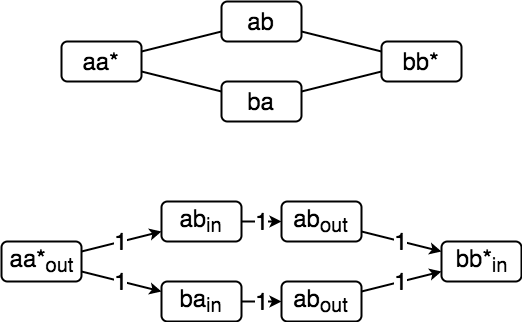
\includegraphics[scale=0.4]{120523-9b.png}
\end{task}

\subsection*{Computational complexity}

\begin{task}{10. (a)}
	\framebox{B} 
\end{task}

\subsection*{NP-hardness}

\begin{task}{12. (f)}
	\qquad Given an instance of Hamiltonian path, $G=(V,E)$, construct an instance of Manystars, $M$. Let $v\in V$ represent a starred word and for $\{v,u\}\in E$ let $v$ and $u$ be neigbouring words. Given a solution, $T$, to $G$, $T$ is also a solution to $M$.
\end{task}

\pagebreak
\section*{Exam 110525}
\subsection*{Analysis of algorithms}

\begin{task}{1. (a)}
	\framebox{A} $n^2$ is the dominating term, the order is therefore $O(n^2\log n)$.
\end{task}

\begin{task}{(b)}
	\framebox{B} $O(n^{3/2}\log n)$ is smaller than $O(n^2\log n)$.
\end{task}

\begin{task}{(c)}
	\framebox{B} $O(n^{3/2})$ is smaller than $O(n^2\log n)$.
\end{task}

\begin{task}{2. (a)}
	\framebox{D} The \textbf{while}-loop will run for $O(n/2)=O(n)$ which gives a total running time of $O(n^2)$.
\end{task}

\begin{task}{3. (a)}
	\framebox{A} $\abs{S}\leq 1$ which means \textbf{insert} and \textbf{remove} runs in constant time. This gives a totalt running time of $O(n)$.
\end{task}

\begin{task}{(b)}
	\framebox{D} The running time can't be lower than $O(n)$ since that's the run time for the \textbf{for}-loop. 
\end{task}

\begin{task}{4. (a)}
	\framebox{A} The total running time will be the running time of $f(n-1)$, $f(n-3)$ and then constant oprations in the function combined. Therefore $T(n)=T(n-1)+T(n-3)+O(1)$.
\end{task}

\begin{task}{(b)}
	\framebox{C}
\end{task}

\subsection*{Graphs}

\begin{task}{5. (a)}
	\framebox{B}
\end{task}

\begin{task}{(b)}
	\framebox{C}
\end{task}

\begin{task}{(c)}
	\framebox{A} Since there is no cycles it's a tree.s
\end{task}

\begin{task}{(d)}
	\framebox{B} You need to pass through the center node to reach all other nodes.
\end{task}

\begin{task}{(e)}
	\framebox{D} Choose all nodes except the center node.
\end{task}

\subsection*{Greedy}

\begin{task}{6. (a)}
	It will always move north east since this will be the only positive integer.
	
	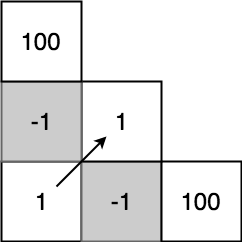
\includegraphics[scale=0.3]{110525-6a.png}
\end{task}

\subsection*{Graph connectivity}

\begin{task}{7. (a)}
	\framebox{C} See \taskref{arg1}
\end{task}

\begin{task}{(b)}
	Let each cell be a node and all valid knight moves be edges. If a white piece is in either end of an edge, remove that edge. Then find a path from the knight to the king by using e.g. BFS.
	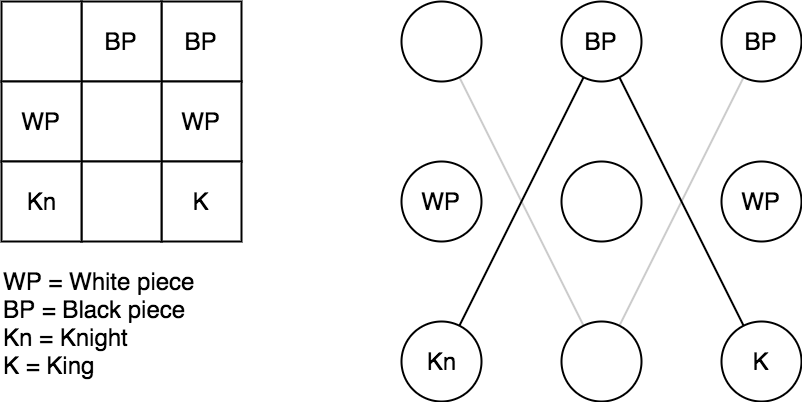
\includegraphics[scale=0.3]{110525-7b.png}
\end{task}

\subsection*{Dynamic programming}

\begin{task}{7. (a)}
	\framebox{C} See \taskref{arg1}
\end{task}



\begin{task}{12. (f)}
	Given an instance of Indendent set, $I$, consisting of $G(V,E)$. and construct an instance of Graphkings, $K$, consisting of $G'(V',E')$ and $k$. Let $G'=G$. Reduction runs in constant time.
	
	If $T\geq k$ is a solution to Graphkings, $T$ is a solution to $K$.
\end{task}

\pagebreak
\section*{Exam 110825}
\subsection*{Analysis of algorithms}

\begin{task}{1. (a)}
	\fbox{A} $n^2$ is the cominating term which means $f(n)=O(n^2)<O(n^2\log n)$.
\end{task}

\begin{task}{(b)}
	\fbox{B} $f(n)=O(n^2)>O(n^{3/2}\log n)$.
\end{task}

\begin{task}{(c)}
	\fbox{B} $f(n)=O(n^2)>O(n^{3/2})$.
\end{task}

\begin{task}{2. (a)}
	\fbox{C} Since $j$ doubles for every iteration the \textbf{while}-loop will run in $\log n$ which means the total running time will be $n\log n$.
\end{task}

\begin{task}{3. (a)}
	\fbox{A} The \textbf{for}-loop runs $n$ times and the inside runs in constant time.
\end{task}

\begin{task}{(b)}
	\fbox{D} The running time can't be smaller than the running time for the \textbf{for}-loop.
\end{task}

\subsection*{Greedy}

\begin{task}{4. (a)}
	\qquad Green represents the optimal route and red represents the route chosen by the greedy algorithm.
	
	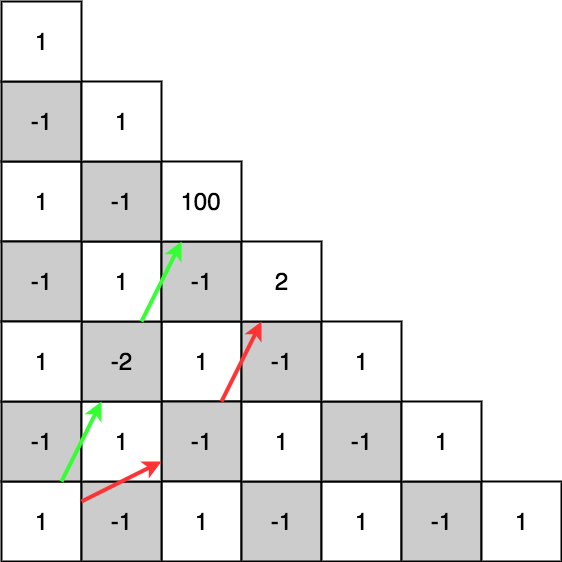
\includegraphics[scale=0.3]{110825-4a.png}
\end{task}

\subsection*{Graph connectivity}

\begin{task}{5. (a)}
	\fbox{C}
\end{task}

\pagebreak
\begin{task}{(b)}
	\qquad Let each number, excluding forbidden numbers, be a node and add an edge between two numbers if all except one of the corresponding digits are equal and the unequal digits lie next to each other on the wheel. Use BFS starting on start until reaching target.
	
	Number of nodes is $10^n-k$ and number of vertices is $O(n(10^n-k))$.
	
	The following example uses $n=2$.
	
\begin{lstlisting}
input:
00 --start
13 --target
89 --nbr of forbidden nodes
01
03
08
14
...
99
\end{lstlisting}
	
	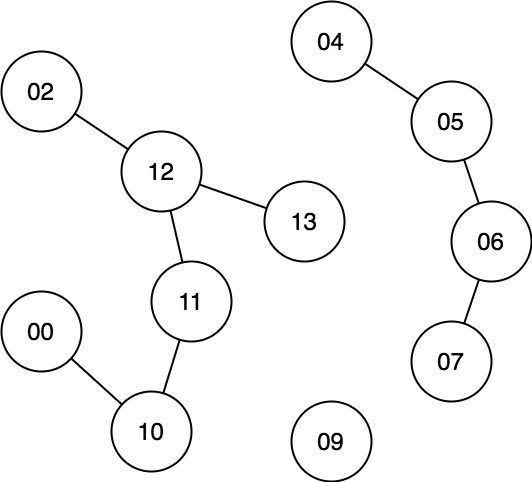
\includegraphics[scale=0.3]{110825-5b.png}
\end{task}

\subsection*{Dynamic programming}

\begin{task}{6. (a)}
	\fbox{B}
\end{task}

\begin{task}{(b)}
	\[\OPT(i,j)=\max\{\OPT(i-1,j-2), \OPT(i-2,j-1)\}+c(i,j)\]
\end{task}

\begin{task}{(c)}
	\qquad The running time and space complexity is $O(n^2)$.
\end{task}

\subsection*{Network flow}

\begin{task}{7. (a)}
	\fbox{A} 
\end{task}

\begin{task}{(b)}
	\qquad 
	\begin{enumerate}
		\item Let $a$ be the source and $b$ the sink.
		\item Replace each vertex, $v$, with $v_{in}$ and $v_{out}$, add the edge $(v_{in},v_{out})$ and change all edges, $(u,v)$, to $(u_{out},v_{in})$.
		\item Set the weight of all edges to 1.
		\item Remove $a_{in}$ and $b_{out}$ and all connected edges since they aren't useful.
	\end{enumerate} 
\end{task}

\subsection*{Computational complexity}

\begin{task}{8. (a)}
	\fbox{A}
\end{task}

\begin{task}{(b)}
	\fbox{A} This seems to be wrong, $v$ isn't relevant.
\end{task}

\begin{task}{(c)}
	\fbox{A}
\end{task}

\begin{task}{(d)}
	\qquad This seems to be wrong, $v$ isn't relevant.
\end{task}

\begin{task}{9. (a)}
	\qquad Since the question seems to be wrong, no answer is given.
\end{task}

\begin{task}{(b)}
	\qquad Since the question seems to be wrong, no answer is given.
\end{task}

\begin{task}{(c)}
	\qquad Since the question seems to be wrong, no answer is given.
\end{task}

\subsection*{NP-hardness}

\begin{task}{10. (a)}
	\fbox{D} ChessHate \footnote{The instruction ``Pieces of different types can never be placed on neighbouring vertices'' should be ``Pieces of the same type can never be placed on neighbouring vertices'' according to Thore}
\end{task}

\begin{task}{(b)}
	\fbox{A}
\end{task}

\begin{task}{(c)}
	\fbox{B}
\end{task}

\begin{task}{(d)}
	\fbox{A}
\end{task}

\begin{task}{(e)}
	\fbox{L}
\end{task}

\begin{task}{(f)}
	\qquad Given an instance of Graph colouring, $G=(V,E),\{c_1,c_2,c_3\}$, construct an instance of ChessHate, $C=(V',E')$. Let $(V',E')=(V,E)$ and let $\{c_1,c_2,c_3\}$ represent Rook, Pawn and Knight respectively. Given a solution, $T$, to $G$, $T$ is also a solution to $C$. 
\end{task}

\pagebreak
\section*{Exam 100528}
\subsection*{Analysis of algorithms}

\begin{task}{1. (a)}
	\framebox{A} The dominating term in $(n^2+2n)/n+\frac{1}{1000}n^{3/2}=n+2+\frac{1}{1000}n^{3/2}$ is $\frac{1}{1000}n^{3/2}$ which means $f(n)=O(n^{3/2}\log n)$. $O(n^2\log n)>O(n^{3/2}\log n) \Rightarrow f(n)=O(n^2\log n)$.
\end{task}

\begin{task}{(b)}
\framebox{A} See \taskref{(a)}.
\end{task}

\begin{task}{(c)}
	\framebox{B} $O(n^{3/2})<O(n^{3/2}\log n) \Rightarrow f(n)\neq O(n^{3/2})$.
\end{task}

\begin{task}{2. (a)}
	\framebox{C} The \textbf{while}-loop runs for $O(\log n)$ and the \textbf{for}-loop for $O(n)$ which gives a total running time of $O(n\log n)$.
\end{task}

\begin{task}{3. (a)}
	\framebox{A} The upper bound can clearly be set to $O(n\log n)$ (if $\abs{S}=n$ is true for every iteration in both loops the running time will be $O(n\log n)$). Since $\abs{S}\leq n$ the running time is at most $O(n\log n)$. No option is smaller than that.
\end{task}

\begin{task}{(b)}
	\framebox{A} If either \textbf{insert} or \textbf{remove} has $O(log\abs{S})$ that loop will run in $O(n\log n)$ because $\abs{S}=n$ in between the loops which means one of the loops wont run in linear time.
\end{task}

\begin{task}{4. (a)}
	\framebox{A} The running time will be the running time of $T(n-1)$, $T(n-3)$ and the constant opreations, $O(1)$, combined.
\end{task}

\begin{task}{(b)}
	\framebox{C} 
\end{task}

\begin{task}{(c)}
	\framebox{C} Since the problem is halved for every step in the recursion $T(n)$ will be called $O(\log n)$ times. This means the total running time will be $O(\log n \* n\log^2 n)=O(n\log^3 n)$.
\end{task}

\subsection*{Graphs}

\begin{task}{5. (a)}
	\framebox{A}
\end{task}

\begin{task}{(b)}
	\framebox{A} There is $r-1$ edges from $v_1$ and there is $r-1$ edges between $v_2,\ldots,v_r$ which is a total of $r+1+r+1=2r+2$.
\end{task}

\begin{task}{(c)}
	\framebox{B} A tree can't contain cycles.
\end{task}

\begin{task}{(d)}
	\framebox{A} Start in $v_1$ and go to all the nodes in numerical order then go from $v_r$ to $v_1$, this as a Hamiltonian cycle.
\end{task}

\begin{task}{(e)}
	\framebox{C} You can choose every second node of $v_2,\ldots,v_r$ (if $r$ is even there will be two adjacent nodes that are not in the set, this is dealt with by using the floor ($\lfloor \rfloor$) function). 
\end{task}

\subsection*{Greedy}

\begin{task}{6. (a)}
	\framebox{A} Sell! Sort the columns by the number of flowers in them and choose the $k$ columns with the most number of flowers. 
\end{task}

\begin{task}{(b)}
	\framebox{B} See \taskref{(a)}.
\end{task}

\begin{task}{(c)}
	\framebox{B} See \taskref{(a)}.
\end{task}

\begin{task}{(d)}
	\framebox{A} See \taskref{(a)}.
\end{task}

\begin{task}{(e)}
	\framebox{A} At first build a heap-based priority queue by finding the numbers of flowers in current cloumn (takes $O(n)$) and add it to the queue (takes $O(m)$) which gives a total running time of $O(nm)$. Then extract $k$ elements (takes $O(k\log m)$). The combined running time is therefore $O(nm+k\log n)$.
\end{task}

\subsection*{Dynamic programming}

\begin{task}{7. (a)}
	\framebox{B} Square
\end{task}

\begin{task}{(b)}
	\framebox{A} It needs to be dependent on whether or not there's a flower at the current position (\framebox{A},\framebox{B},\framebox{F}) and return 0 if there's no flower (\framebox{A}).
\end{task}

\begin{task}{(c)}
	\framebox{C} You need to pass each nposition exactly once, hence $O(nm)$.
\end{task}

\begin{task}{(d)}
	\framebox{C} You need to save a constant amount of data for each position.
\end{task}

\subsection*{Network flow}

\begin{task}{8. (a)}
	\framebox{D} Dance, see \taskref{(d)}.
\end{task}

\begin{task}{(b)}
	\framebox{A} See \taskref{(d)}.
\end{task}

\begin{task}{(c)}
	\framebox{A} See \taskref{(d)}.
\end{task}

\begin{task}{(d)}
	\qquad You have two columns of nodes, let each node in the first represent a row and each node in the second represent a column. Insert an directed edge from a row-node to a column-node if they have a flower in common. Add a source with directed edges to each node in the first column. Add a sink with directed edges from each node in the second column. Set the weight of all edges to 1.
	
	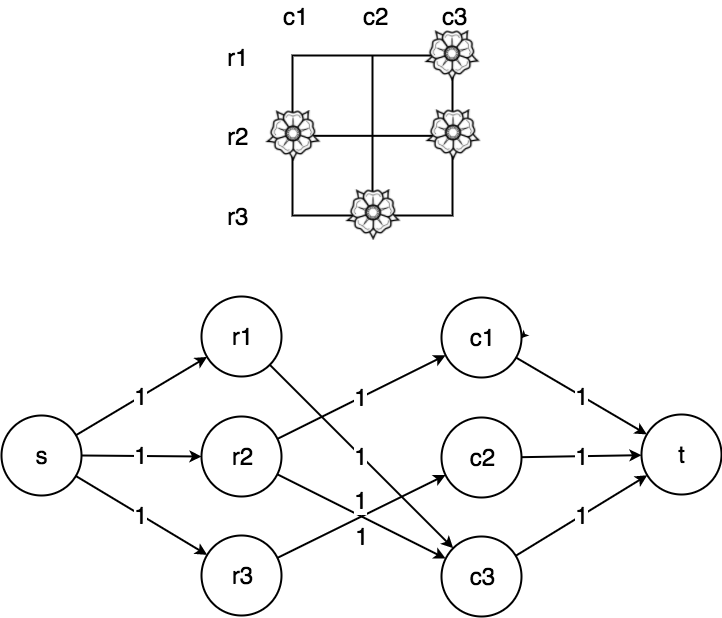
\includegraphics[scale=0.3]{100528-8d.png}
	
	If the maximum flow through the network is greater than or equal to $k$ then there is a solution.
\end{task}

\subsection*{Computational complexity}

\begin{task}{9. (a)}
	\framebox{A}
\end{task}

\begin{task}{(b)}
	\framebox{B}
\end{task}

\begin{task}{(c)}
	\framebox{A}
\end{task}

\begin{task}{(d)}
	\framebox{A}
\end{task}

\begin{task}{10. (a)}
	\framebox{C}
\end{task}

\begin{task}{(b)}
	\framebox{D}
\end{task}

\begin{task}{(c)}
	\framebox{B}
\end{task}

\subsection*{NP-hardness}

\begin{task}{11. (a)}
	\framebox{C} EU, it's the same problem as set cover since you can see each column as a set where each element is the flowers corresponding rows, you need to find minimum set cover and return all other columns.
\end{task}

\begin{task}{(b)}
	\framebox{D}
\end{task}

\begin{task}{(c)}
	\framebox{B}
\end{task}

\begin{task}{(d)}
	\framebox{D}
\end{task}

\begin{task}{(e)}
	\framebox{K}
\end{task}

\begin{task}{(f)}
	\qquad Given an instance of Set Cover, $C$, consisting of a set of sets, $S$, construct an instance of EU, $E$. Let $S_i\in S$ represent a column in $E$ and $s_j\in S_i$ a flower where column $i$ and row $j$ meets. Given a solution, $T$, to $C$, $S \setminus T$ is a soltion to $E$.
\end{task}




\begin{task}{100107 12. (f)}
	\qquad Given an instance of Hamiltonian cycle, $G=(V,E)$, construct an instance of Hyperspace. We represent $v\in V$ with a star. For $v$ and $u$ where $\{v,u\}\not\in E$ we place a space danger in between the corresponding stars. If there is a cycle that visits each star exactly once, $G$ is Hamiltonian.
\end{task}
\end{document}